%
%   K A D O N O
%   "kadono.tex"
%

\documentclass[10pt,b5paper,papersize,dvipdfmx]{jsbook}

\usepackage{vuccaken}
\usepackage{vuccaken2019}

% スタイルファイルの読み込みや自作マクロは、
% 最終的には vuccaken2019.sty の中に書いてください。
% とりあえずはここに書いてもらって構いません。


\begin{document} % 以下本文

% - - - - - - - - - - - - - - - - - - - - - - - - %
\kaishititle%
  {熱}% title
  {物理科学 M1}% 所属
  {門野広大}% name
% - - - - - - - - - - - - - - - - - - - - - - - - %

% \setcounter{tocdepth}{2} % 目次にどこまで表示するか
% \tableofcontents % 目次出力
% \clearpage % 改ページ

\section*{はじめに}
熱って何?温度ってなに?どうやって熱は伝わっているの?そんな疑問に一生に一度は出会ったことがあると思います。実際熱の伝わり方というものをちゃんと理解しようとすると莫大な時間がかかりますし、不可逆なものでもあるのでそもそも理解できないのかもしれません。でも、限定的な条件において理解することは容易にできます。今回の会誌ではそんな物理の世界では常識的なことを主に書いていきたいと思います。\par
今回は状況が限定的な状態で、実際に人間が住んでいる環境とはかけ離れているため役に立たないと思われると思います。研究分野ではとても役にたちます。その理由を最後の方に私がやっている研究の話を含めて書きたいと思います。

% 熱って何?そもそも温度って何?熱伝導率って何で決まるの?物質のなに?格子ってなに?
% 格子振動って何?フォノンってなに?

%
\section{温度}



\section{フォノン君}
固体の熱の伝わり方を考えていくため格子ということについて考えていく必要があります。


\section{比熱とか熱伝導率とか}

\section{ちょっと変わった話}

\section{終わりに}
% \begin{figure}[htbp]
%   \centering
%   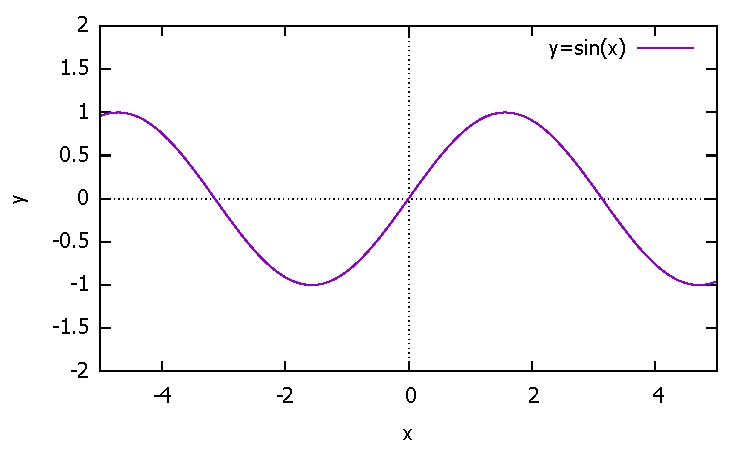
\includegraphics[width=10cm]{temp/fig-sin.pdf}
%   \caption{$y=\sin x$のグラフ。gnuplotで作成した。}
%   \label{fig:sin}
% \end{figure}

%% 参考文献
\begin{sanko}
  \begin{enumerate}
    \item W.COCHRAN 著 小林正一、福地充 訳 固体物性シリーズ3格子振動 丸善出版 (昭和50年)
    \item 田崎晴明 著 新物理学シリーズ37統計力学 培風館 (2008)
  \end{enumerate}
\end{sanko}


\end{document}
%
% ファイトだよ!
%